\documentclass[12pt, notitlepage, final]{article}

\newcommand{\name}{Vince Coghlan}

%\usepackage[dvips]{graphics,color}
\usepackage{amsfonts}
\usepackage{amssymb}
\usepackage{amsmath}
\usepackage{latexsym}
\usepackage{enumerate}
\usepackage{amsthm}
\usepackage{nccmath}
\usepackage{setspace}
\usepackage[pdftex]{graphicx}
\usepackage{epstopdf}
\usepackage[siunitx]{circuitikz}
\usepackage{tikz}
\usepackage{float}
\usepackage{cancel}
\usepackage{setspace}
\usepackage{overpic}
\usepackage{mathtools}
\usepackage{listings}
\usepackage{color}
\usepackage{qtree}
\usepackage{gensymb}

\usetikzlibrary{calc}
\usetikzlibrary{matrix}
\usetikzlibrary{positioning}

\numberwithin{equation}{section}
\newcommand{\dbr}[1]{d_{\mbox{#1BR}}}
\newtheorem{lemma}{Lemma}
\newtheorem*{corollary}{Corollary}
\newtheorem{theorem}{Theorem}
\newtheorem{proposition}{Proposition}
\theoremstyle{definition}
\newtheorem{define}{Definition}

\newdimen\digitwidth{}
\settowidth\digitwidth{0}
\def~{\hspace{\digitwidth}}

\setlength{\parskip}{1pc}
\setlength{\parindent}{0pt}
\setlength{\topmargin}{-3pc}
\setlength{\textheight}{9.0in}
\setlength{\oddsidemargin}{0pc}
\setlength{\evensidemargin}{0pc}
\setlength{\textwidth}{6.5in}
\newcommand{\answer}[1]{\newpage\noindent\framebox{\vbox{{\bf CSCI 3753 Spring 2014} 
\hfill {\bf \name} \vspace{-1cm}
\begin{center}{Homework \#3}\end{center} } }\bigskip }

\DeclareMathOperator*{\argmin}{arg\,min}

%absolute value code
\DeclarePairedDelimiter\abs{\lvert}{\rvert}%
\DeclarePairedDelimiter\norm{\lVert}{\rVert}
\makeatletter
\let\oldabs\abs{}
\def\abs{\@ifstar{\oldabs}{\oldabs*}}
%
\let\oldnorm\norm{}
\def\norm{\@ifstar{\oldnorm}{\oldnorm*}}
\makeatother

\def\dbar{{\mathchar'26\mkern-12mu d}}
\def\Frac{\displaystyle\frac}
\def\Sum{\displaystyle\sum}
\def\Int{\displaystyle\int}
\def\Prod{\displaystyle\prod}
\def\P[x]{\Frac{\partial}{\partial{} x}}
\def\D[x]{\Frac{d}{dx}}
\newcommand{\PD}[2]{\frac{\partial#1}{\partial#2}}
\newcommand{\PF}[1]{\frac{\partial}{\partial#1}}
\newcommand{\DD}[2]{\frac{d#1}{d#2}}
\newcommand{\DF}[1]{\frac{d}{d#1}}
\newcommand{\fix}[2]{\left(#1\right)_#2}
\newcommand{\ket}[1]{|#1\rangle}
\newcommand{\bra}[1]{\langle#1|}
\newcommand{\braket}[2]{\langle{} #1 | #2 \rangle}
\newcommand{\bopk}[3]{\langle{} #1 | #2 | #3 \rangle}
\newcommand{\Choose}[2]{\displaystyle{} {#1 \choose{} #2}}
\newcommand{\proj}[1]{\ket{#1}\bra{#1}}
\def\del{\vec{\nabla}}
\newcommand{\avg}[1]{\langle#1\rangle}
\newcommand{\piecewise}[4]{\left\{\beginProtected{array}{rl}#1&:#2\\#3&:#4\endProtected{array}\right.}
\newcommand{\systeme}[2]{\left\{\beginProtected{array}{rl}#1\\#2\endProtected{array}\right.}
\def\KE{K\!E}
\def\Godel{G$\ddot{\mbox{o}}$del}

\onehalfspacing{}

\begin{document}

\answer{}

\begin{figure}[H]
\begin{center}
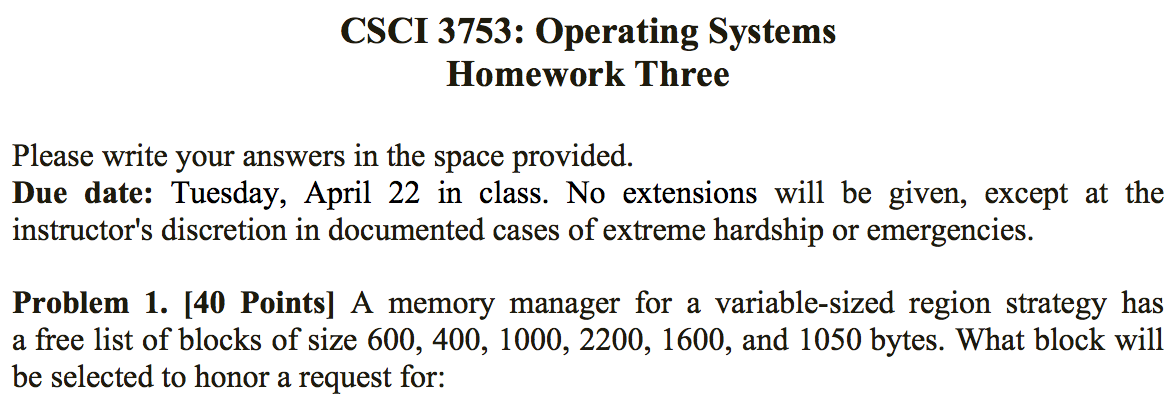
\includegraphics[width=14cm]{f1}
\end{center}
\end{figure}

\begin{enumerate}[(a)]
  \item{1603 bytes using a best-fit policy?}\\
    2200
  \item{949 bytes using a best-fit policy?}\\
    1000
  \item{1603 bytes using a worst-fit policy?}\\
    2200
  \item{349 bytes using a worst-fit policy?}\\
    2200
  \item{1603 bytes using a first-fit policy?}\\
    2200
  \item{1049 bytes using a first-fit policy?}\\
    2200
\end{enumerate}

\begin{figure}[H]
\begin{center}
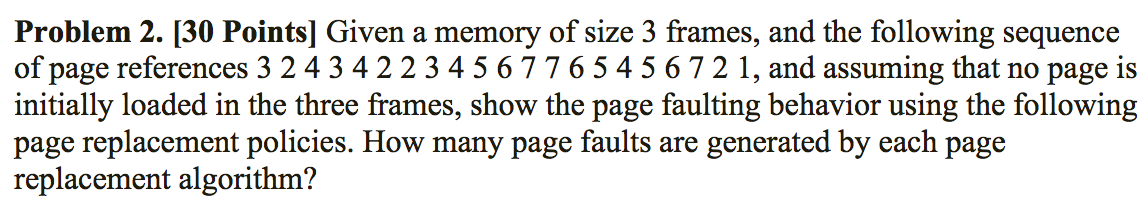
\includegraphics[width=14cm]{f2}
\end{center}
\end{figure}
\begin{enumerate}[(a)]
  \item{FIFO}\\
    \begin{tabular}{ c c c c c c c c c c c c }
      3 & 3 & 3 & 5 & 5 & 5 & 4 & 4 & 4 & 7 & 7 & 7 \\
        & 2 & 2 & 2 & 6 & 6 & 6 & 5 & 5 & 5 & 2 & 2 \\
        &   & 4 & 4 & 4 & 7 & 7 & 7 & 6 & 6 & 6 & 1 \\
    \end{tabular}\\
    Thats 12 faults.
  \item{OPT}\\
    \begin{tabular}{ c c c c c c c c c c c c }
      3 & 3 & 3 & 5 & 5 & 5 & 5 & 7 & 7 \\
        & 2 & 2 & 2 & 6 & 6 & 6 & 6 & 2 \\
        &   & 4 & 4 & 4 & 7 & 4 & 4 & 1 \\
    \end{tabular}\\
    Thats 9 faults.
  \item{LRU}\\
    \begin{tabular}{ c c c c c c c c c c c c }
      3 & 3 & 3 & 3 & 6 & 6 & 6 & 6 & 6 & 1 \\
        & 2 & 2 & 5 & 5 & 5 & 5 & 5 & 2 & 2 \\
        &   & 4 & 4 & 4 & 7 & 4 & 7 & 7 & 7 \\
    \end{tabular}\\
    Thats 10 faults.
\end{enumerate}

\begin{figure}[H]
\begin{center}
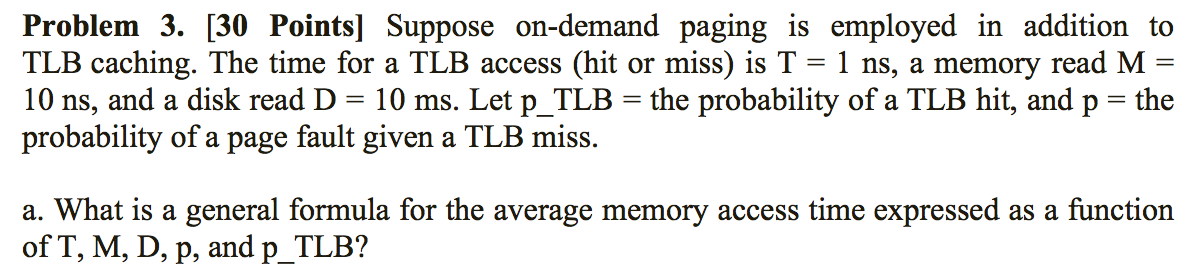
\includegraphics[width=14cm]{f3}
\end{center}
\end{figure}

\[
  p\_TLB\cdot T  + (1-p\_TLB)\cdot p\cdot (T + M) + (1-p\_TLB)(1-p)(T + M + D)
\]

\begin{figure}[H]
\begin{center}
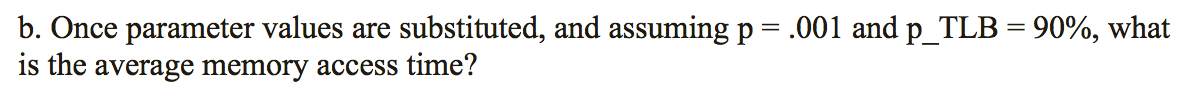
\includegraphics[width=14cm]{f4}
\end{center}
\end{figure}
\[
  t = 0.999ms \approx 1ms
\]

\end{document}

